%%%%%%%%%%%%%%%%%%%%%%%%%%%%%%%%%%%%%%%%%%%%%%%%%%%%%%%%%%%%%%%%%%%%%%%%%%%%%%%%
%neutrino_physics.tex: Chapter on neutrino physics:
%%%%%%%%%%%%%%%%%%%%%%%%%%%%%%%%%%%%%%%%%%%%%%%%%%%%%%%%%%%%%%%%%%%%%%%%%%%%%%%%
\chapter{Theoretical Motivations}
\label{wrBosonAndHeavyNu}
%%%%%%%%%%%%%%%%%%%%%%%%%%%%%%%%%%%%%%%%%%%%%%%%%%%%%%%%%%%%%%%%%%%%%%%%%%%%%%%%
Experimental evidence of massive neutrinos motivates extensions to the ST.  Neutrino flavor oscillations have 
been observed by experiments \cite{kamiokandeTwo,solarNuSummary,NOvAresults,mainzPhaseIIResults,t2kResults,dayaBayResults}, 
and these observations imply that neutrinos have mass.  Neutrinos in the ST are only produced in left-handed 
states, so an extension, like the LRS model, with massive neutrinos is needed for a Lorentz invariant theory.

In this chapter, particle mass generation is discussed as a precursor to ST extensions; 
then, the Majorana neutrino model and the LRS model are explained, highlighting how these extensions 
show better agreement with experimental observations than the ST.  In conclusion, 
important characteristics of the LRS model that can be studied at the LHC are presented.


\section{Particle Masses in the Standard Theory}
\label{sec:massInSM}
In the ST the Brout-Englert-Higgs (BEH) mechanism transforms the four $SU(2)_{L} \times U(1)$ group 
generators into the electroweak interaction mediators.  The BEH mechanism 
introduces a complex doublet $\Phi$, representing four scalar bosons, that obey the Lagrangian $\Ell_{H}$:

\begin{align}
	\Phi &= \begin{bmatrix}
	\phi^{+} \\
	\phi^{0}
	\end{bmatrix}
\end{align}

\begin{equation}
	\Ell_{H} = (D_{\mu}\Phi)^{\dagger}D^{\mu}\Phi - V(\Phi)
\end{equation}
where $V(\Phi) = \frac{1}{2}(|\Phi|^{2} - \frac{\nu^{2}}{2})$ is the Higgs potential (shown in Figure \ref{fig:smHiggsPotential}), and 
$D_{\mu} = \partial_{\mu} + ig_{L}\tau^{j}A^{j}_{\mu} + i\frac{g'}{2}YB_{\mu}$, represents the propagation 
of the Higgs doublet $\Phi$ and its couplings to the $SU(2)_{L}$ and $U(1)$ generators $\tau^{j}$ and $Y$, 
and to the massless vector fields $A^{j}_{\mu}$ and $B_{\mu}$.  $g_{L}$ and 
$g'$ set the weak and electromagnetic interaction coupling strengths.  The Higgs doublet $\Phi$ naturally 
adopts a value $<\Phi> =$ (0  $\nu/\sqrt{2}$) that minimizes the Higgs potential, after which $\Ell_{H}$ reduces 
to:

\begin{figure}[h]
	\centering
	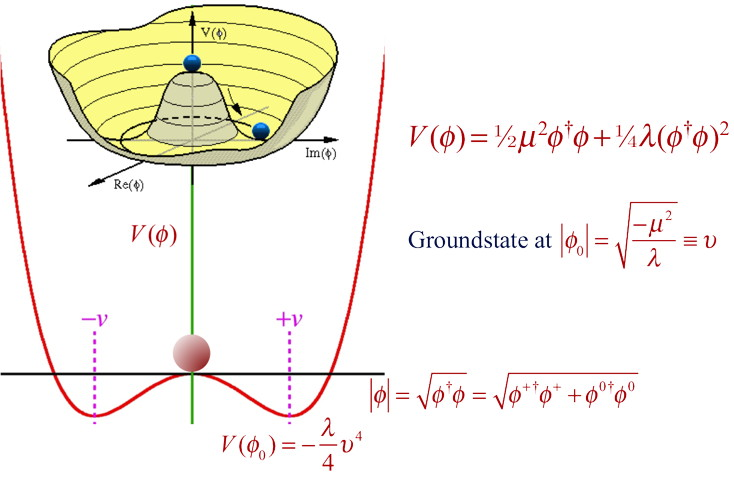
\includegraphics[width=1.0\textwidth]{figures/mexicanHatPotential.jpg}
	\caption{The Higgs potential drives the ST Higgs field to a stable state with non-zero vacuum expectation value, from $Swiss Physical Society$ \cite{higgsPotential}.}
	\label{fig:smHiggsPotential}
\end{figure}

\begin{equation}
	\Ell_{HK} = \frac{\nu^{2}}{8}[g^{2}_{L}(A^{1}_{\mu} + iA^{2}_{\mu})(A^{1\mu} - iA^{2\mu}) + (g'B_{\mu} - g_{L}A^{3}_{\mu})^{2}]
	\label{eq:stWeakBosonMassLagrangian}
\end{equation}
Defining the photon vector field $A_{\mu}$, and the weak boson vector fields $W^{\pm}_{\mu}$ and $Z_{\mu}$ as:

\begin{equation}
	W^{\pm}_{\mu} \equiv \frac{1}{\sqrt{2}}(A^{1}_{\mu} \pm iA^{2}_{\mu}), 
	Z_{\mu} \equiv \frac{1}{\sqrt{g'^{2} + g^{2}_{L}}}(g'B_{\mu} - g_{L}A^{3}_{\mu}), 
	A_{\mu} \equiv \frac{1}{\sqrt{g'^{2} + g^{2}_{L}}}(g_{L}B_{\mu} + g'A^{3}_{\mu})
\end{equation}
transforms $\Ell_{HK}$ (Equation \ref{eq:stWeakBosonMassLagrangian}) into:

\begin{equation}
	\Ell_{HK} = (\frac{\nu g_{L}}{2})^{2}W^{+}_{\mu}W^{-\mu} + \frac{1}{2}(\frac{\nu \bar{g}}{2})^{2}Z_{\mu}Z^{\mu} + 0A_{\mu}A^{\mu}
\end{equation}
where $\bar{g} \equiv \sqrt{g'^{2} + g^{2}_{L}}$.  Following from this Lagrangian, the photon $A_{\mu}$ is massless, 
the $Z$ boson has mass $m_{Z} = \nu\bar{g}/2$, and the $W^{\pm}$ bosons have mass $m_{W} = \nu g_{L}/2$.  
Three of the four scalar fields introduced by the BEH mechanism are consumed to give mass to the $Z$ 
and $W^{\pm}$ bosons.  The fourth scalar field manifests as a scalar boson, the Higgs boson, and couples to all 
massive particles with coupling strength proportional to the particle's mass.  Recent experimental evidence 
of the Higgs boson \cite{combinedHiggsResult} supports the ST prediction that the $Z$ and $W^{\pm}$ bosons acquire 
mass through the BEH mechanism.

In the ST, fermions (quarks and leptons) acquire mass by adding more scalar Higgs fields to the 
BEH mechanism.  Additional Higgs fields add mass terms of the form $-mf\bar{f}$, where $f$ is a fermion, to 
the Lagrangian.  In the basis where a fermion field $f$ consists of right- and left-handed components $\chi_{R}$ 
and $\chi_{L}$, $f = (\chi_{L},\chi_{R})$, a fermion mass term in the Lagrangian is expressed as:

\begin{equation}
	\Ell_{D} = -m\bar{f}f = -m\chi^{\dagger}_{L}\chi_{R} - m\chi^{\dagger}_{R}\chi_{L}
	\label{eq:diracMass}
\end{equation}
This type of mass term, called a Dirac mass, contains the product of left- and right-handed fields.  Experimentally, 
quarks and charged leptons exist in left and right-handed states that are degenerate 
in mass, so Dirac mass terms are used to give mass to the fermions in the ST.

Neutrinos play a special role in the ST, where they are neutral, massless fermions, that only interact 
through the weak interaction.  In addition, due to parity violation of the weak interaction, 
anti-neutrinos are always right-handed, and neutrinos are always left-handed.  In the ST the only mechanism 
to assign masses to fermions is via the Dirac mass term (Equation \ref{eq:diracMass}), which depends on the 
product of left- and right-handed fields.  As the Dirac mass term for a neutrino yields a mass of zero, an 
extension is required to account for the experimental observation of massive neutrinos.


\section{Standard Theory Extensions}
\label{sec:lrsExtensions}
There are several ways that the ST can be extended to accommodate massive, fermionic neutrinos.  In one of the 
simplest extensions neutrinos are not Dirac fermions, but Majorana fermions, which are their own anti-particles 
and have masses, $m_{L},m_{R}$, defined in the Lagrangian $\Ell_{M}$ -

\begin{equation}
	\Ell_{M} = -m_{L}\chi^{\dagger}_{L}\chi_{L} - m_{R}\chi^{\dagger}_{R}\chi_{R}
\end{equation}
The individual Majorana masses are generated through an extended Higgs model.  Another consequence of Majorana 
neutrinos would allow neutrinoless double beta decays to occur.  This has not yet been observed \cite{igexDblBetaDecay,gerdaDblBetaDecay} 
leading to the exploration of alternate ideas.

An alternative is the Left-Right Symmetric (LRS) model, which predicts massive fermionic neutrinos, but has not 
yet been observed in experiments.
First proposed in 1974 \cite{earlyLRSModel}, the LRS model predicts an electroweak 
interaction existed in the very early universe, which conserved parity and was mediated by seven massless 
gauge bosons.  An extension of the ST BEH mechanism transformed the seven massless gauge bosons 
into the ST electroweak bosons, and the heavier $W^{\pm}_{R}$ (\WR) and $Z'$ bosons.

In the LRS model an $SU(2)_{R}$ group is added to the ST electroweak $SU(2)_{L} \times U(1)$ groups.
This introduces three massless vector fields $\xi^{j}_{R\mu}$, which become massive 
bosons through an extended version of the BEH mechanism.  The extension is in two stages and 
ultimately yields one massless and six massive gauge bosons that mediate the electroweak interactions.  
In the first stage \cite{lrsHiggsStageOne}, a chiral, complex Higgs doublet $\chi_{L,R}$ is introduced: 

\begin{align}
	\chi_{L,R} &= \begin{bmatrix}
	\chi^{+}_{L,R} \\
	\chi^{0}_{L,R}
	\end{bmatrix}
	\label{eq:stageOneVEV}
\end{align}
with bosonic fields that couple independently to the left- and right-handed gauge bosons.  The propagation and 
interaction of these new fields with other massless bosons is described by the Lagrangian:

\begin{equation}
	\Ell_{H,LRS} = \frac{1}{2}(D_{\mu}\chi_{L})^{\dagger}D^{\mu}\chi_{L} + \frac{1}{2}(D_{\mu}\chi_{R})^{\dagger}D^{\mu}\chi_{R} - V(\chi_{L,R})
	\label{eq:stageOneHiggsLrs}
\end{equation}
where $D_{\mu} = \partial_{\mu} + ig_{L}\tau^{j}A^{j}_{L\mu} + ig_{R}\tau^{j}\xi^{j}_{R\mu} + i\frac{g'}{2}YB_{\mu}$ contains 
the massless boson fields $A^{j}_{L\mu}, \xi^{j}_{R\mu}, B_{\mu}$ multiplied by the generators of the $SU(2)_{L}, SU(2)_{R}, U(1)$ groups.  
In the model considered here the coupling strengths $g_{R}, g_{L}$ were assumed to be equal, and denoted as $g$.  
The potential $V(\chi_{L,R})$ respects the LRS model symmetries, and depends on a constant, $U_{R}$.  $\chi_{L,R}$ 
equilibrated at $<\chi^{+}_{L,R}> = 0, <\chi^{0}_{L}> = 0, <\chi^{0}_{R}> = U_{R}$ to minimize $V(\chi_{L,R})$, 
and subsequently creating new fields:

\begin{equation}
	W^{\pm}_{R\mu} \equiv \frac{1}{\sqrt{2}}(\xi^{1}_{R\mu} \mp i\xi^{2}_{R\mu}), 
	Z'_{\mu} \equiv \frac{1}{\sqrt{g'^{2} + g^{2}}}(-g'B_{\mu} + g\xi^{3}_{R\mu})
\end{equation}
with masses given by:

\begin{equation}
	\mWR = \frac{1}{2}gU_{R}  \quad m_{Z'} = \frac{1}{2}U_{R}\sqrt{g'^{2} + g^{2}}
\end{equation}
After the first stage, the $\WR$ and $Z'$ bosons are predicted to have masses $\mWR = \frac{1}{2}gU_{R}$ and 
$m_{Z'} = \frac{1}{2}U_{R}\sqrt{g'^{2} + g^{2}}$, and all other bosons remain massless.

In the second stage \cite{lrsHiggsStageOne,lrsHiggsStageTwo} two complex Higgs doublets $\phi_{1}$ and $\phi_{2}$ 
are introduced, and are represented by the multiplet $\Phi$:

\begin{align}
	\Phi &= \begin{bmatrix}
	\phi^{0}_{1} & \phi^{+}_{2} \\
	\phi^{-}_{1} & \phi^{0}_{2}
	\end{bmatrix}
\end{align}
This multiplet interacts with the left- and right-handed $SU(2)$ boson fields, and these interactions obey a Lagrangian 
$\Ell_{H2,LRS}$ similar to Equation \ref{eq:stageOneHiggsLrs} but with additional terms for the second Higgs doublet.  
Within $\Ell_{H2,LRS}$ is a potential $V(\phi_{1},\phi_{2})$, and $\Phi$ naturally adopts a non-zero expectation 
value that minimizes $V(\phi_{1},\phi_{2})$:

\begin{align}
	<\Phi> &= \begin{bmatrix}
	\nu_{1} & 0 \\
	0 & \nu_{2}
	\end{bmatrix}
	\label{eq:stageTwoVEV}
\end{align}
At equilibrium, the \WR, $Z'$, and the ST $W^{\pm}$ and $Z$ bosons have acquired masses given by:

\begin{equation}
	m_{W} = \frac{1}{2}g\nu ,\quad m_{W_{R}} \simeq \frac{1}{2}gU_{R} ,\quad m_{Z} = \frac{1}{2}\bar{g}\nu ,\quad m_{Z'} \simeq \frac{1}{2}\bar{g}U_{R}
\end{equation}
\begin{equation}
	\nu^{2} \equiv \nu^{2}_{1} + \nu^{2}_{2} , \quad \bar{g}^{2} \equiv g^{2} + g'^{2}
\end{equation}
The assumptions are that $U_{R} \gg \nu$, and there is negligible mixing between the left and right-handed leptons.  
Thus, the LRS model predicts the correct masses for the ST weak bosons, and masses for three new, heavier bosons.  
The mass splitting between the left-handed $W^{\pm},Z$ and the right-handed $\WR,Z'$ is an indication of parity 
violation in the LRS model, as compared with the ST without a clear theoretical motivation.  In the fermionic sector, 
the LRS model predicts new neutrinos with masses consistent with neutrino flavor oscillations.

With the addition of the $SU(2)_{R}$ group, three new right-handed neutrinos $N^{l}_{R}$ (\nul) arise naturally 
to form doublets of $SU(2)_{R}$ hypercharge with right-handed charged leptons.  The LRS model 
predicts non-zero masses for \nul and ST neutrinos using a mixture of Dirac and Majorana mass terms \cite{seeSawAndParityViolation,seeSawAndGUTs}:

\begin{align}
	\Ell &= \frac{1}{2}(\bar{\nu}_{Li} \quad \bar{\nu}_{Ri})\begin{bmatrix}
	B'_{i} & M_{i} \\
	M_{i} & B_{i}
\end{bmatrix}(\nu_{Li} \quad \nu_{Ri})^{T}
\label{eq:nuMasses}
\end{align}
where $i$ is the lepton generation, and $\nu_{L}$ and $\nu_{R}$ are massive, pure left and right-handed 
fermionic neutrino fields.  The nonzero value of $<\Phi>$ in equation \ref{eq:stageTwoVEV} yields the 
Dirac masses $M_{i}$, and the expectation values of $\chi_{L}$ and $\chi_{R}$ defined in equation \ref{eq:stageOneVEV} 
lead to the Majorana masses $B'_{i}$ and $B_{i}$.  Furthermore, $M_{i} \sim \nu$, $B'_{i} \sim 0$, 
$B_{i} \sim U_{R}$, and $B_{i} \gg M_{i}$, which is consistent with $m_{W_{R}} \gg m_{W}$.  Substituting 
$\nu$ and $U_{R}$ for the Dirac and Majorana masses, equation \ref{eq:nuMasses} is diagonalized and yields 
the following neutrino mass eigenvalues, assuming negligible left-right mixing:

\begin{equation}
	\lambda_{i+} \simeq B_{i},  \quad \lambda_{i-} \simeq \frac{M^{2}_{i}}{B_{i}}
\end{equation}
The detectable states $N_{i}$ and $\nu_{i}$ that participate in electroweak interactions are mixtures of the pure 
left- and right-handed neutrino fields:

\begin{equation}
	\nu_{i} \simeq \frac{1}{\sqrt{M^{2}_{i} + B^{2}_{i}}}(B_{i}\nu_{Li} - M_{i}\nu_{Ri}) \simeq \nu_{Li} - \frac{M_{i}}{B_{i}}\nu_{Ri}
	
	N_{i} \simeq \frac{1}{\sqrt{M^{2}_{i} + B^{2}_{i}}}(M_{i}\nu_{Li} + B_{i}\nu_{Ri}) \simeq \nu_{Ri} + \frac{M_{i}}{B_{i}}\nu_{Li}
\end{equation}
with masses given by:

\begin{equation}
	m_{\nu_{i}} = \lambda_{i-} \simeq \frac{M^{2}_{i}}{B_{i}} , \quad m_{N_{i}} = \lambda_{i+} \simeq B_{i}
\end{equation}
Thus, the LRS model predicts the left-handed neutrinos $\nu_{i}$ have masses $\lambda_{i-} \simeq M_{i}\frac{M_{i}}{B_{i}}$, 
and the right-handed neutrinos $N_{i}$ have masses $\lambda_{i+} \simeq B_{i} \gg M_{i}$.  Appropriate choices 
for $M_{i}$ and $B_{i}$ yields very light left-handed neutrinos, very heavy right-handed neutrinos, 
and negligible mixing between left- and right-handed states (suppressed by $\sim \frac{M_{i}}{B_{i}} \ll 1$), 
which is consistent with the experimental evidence \cite{dZeroMixingLimits,theoreticalMixingLimits}.

In addition to predicting massive neutrinos and parity violation in the weak interaction, the LRS model accounts 
for the observed baryon-antibaryon asymmetry of the universe, which the ST does not \cite{surveyOfExtensions}.  
The LRS model predicts a greater degree of CP violation due to the CP violating interactions that are mediated by 
the \WR and $Z'$ bosons, and hence predicts the observed baryon asymmetry.


\section{LRS Model Phenomenology}
\label{sec:lrsPhenomenology}
%WR mass is equal to the product of the SU(2)_{R} coupling constant g and the extended Higgs mechanism 
%electroweak energy scale U_{R} divided by 2.  WR mass must be well above W boson mass, otherwise the Higgs 
%boson branching fraction to WW would deviate from ST predictions
%the heavy nu mass is equal to a mass B generated by the extended Higgs mechanism, and its upper limit 
%is constrained by the sum of all three neutrino masses of ~0.5 eV
%the other unknown parameters of the LRS model is the right-handed analogue of the CKM matrix, which 
%has 3 unknown mixing angles and 1 unknown CP violating phase
%new EWK physics is needed, otherwise, based on the top quark and higgs boson masses, the ST electroweak 
%vacuum would be unstable at an energy scale betwen 10^10 and 10^14 GeV.  heavy neutrinos contribute 
%to negative vacuum stability (unstable), while WR bosons contribute to positive vacuum stability (stable)
%the WR and N masses must be below approximately 10^6.5 GeV, otherwise unitarity is broken at tree level
%see \cite{lrsMassConstraints}


The LRS model discussed thus far retains all the aspects of the ST, and predicts 
massive neutrinos, parity violation in a natural way, and the baryon-antibaryon asymmetry of the universe.  
Specific realizations of the LRS model retain these features, and are distinguished by unique values of 
several free parameters: the weak coupling constant $g_{R}$, the left-right symmetric energy scale $U_{R}$ 
that sets the \WR mass, the masses $B_{i}$ and $M_{i}$ that set the \nul and ST \nu masses, and the three 
mixing angles $\theta_{i}$ and the CP violating phase $\delta_{R}^{CP}$ that define the \WR analogue 
of the CKM quark mixing matrix.  As stated earlier, in this thesis the coupling $g_{R}$ is assumed to be 
the same for all lepton flavors and equal to the ST weak coupling $g_{L}$.  Both the \WR and \nul masses 
are constrained by unitarity to be below $\sim10^{6.5}$ $\GeV$ \cite{lrsMassConstraints}, and the \WR is 
excluded for $\mWR < 2.5$ $\TeV$ based on the neutral kaon $K_{L} - K_{S}$ mass difference \cite{mwrBoundFromNeutralKaons}.  
Not all realizations of the LRS model can be tested at the LHC.  However, at LHC energies there are some 
specific LRS model realizations that can be tested, if the following assumptions are made:

\begin{itemize}
	\item The ST quarks and all right-handed leptons couple to the \WR and $Z'$ with the same strengths 
		as the ST quarks and all left-handed leptons couple to the ST weak bosons.  This constrains the 
		\WR analogue of the CKM matrix to match the ST CKM matrix.
	\item The right-handed neutrinos \nul are lighter than the \WR, and hence the \WR decays to the \nul.
	\item The decay of the \nul does not violate lepton flavor conservation, and hence only the processes 
		$\WR \rightarrow e_{1}N_{e} \rightarrow e_{1}e_{2}W^{*}_{R}$ and $\WR \rightarrow \mu_{1}N_{\mu} \rightarrow \mu_{1}\mu_{2}W^{*}_{R}$ are allowed.
\end{itemize}
Given these assumptions, the \WR and $Z'$ bosons can be produced in proton-proton (pp) collisions delivered by 
the LHC and recorded by the CMS experiment.  The lighter \WR is more likely than the $Z'$ to have a mass within 
the LHC's reach, so LRS model realizations were tested by searching for evidence of the \WR boson.  The \WR 
can decay to a pair of quarks or a charged lepton and heavy neutrino \nul.  The $\WR \rightarrow l\nul$ 
decay channel permits a measurement of the neutrino mass \mnul, and this is the subject of this thesis.


\section{Experimental Signature}
\label{sec:lrsExpSignature}
In the $\WR \rightarrow l_{1}\nul$ channel, the \nul can decay to a virtual $Z'*$ and $\nul^{*}$, or a second 
charged lepton $l_{2}$ and a virtual $\WR^{*}$.  The branching fraction for the \nul decay to detectable particles 
is highest for $\nul \rightarrow l_{2}\WR^{*} \rightarrow l_{2}q_{1}q_{2}$, so the \WR search was conducted in the 
$\WR \rightarrow l_{1}\nul \rightarrow l_{1}l_{2}q_{1}q_{2}$ ($l_{1}l_{2} = ee,\mu\mu$) channel, shown in 
Figure \ref{fig:wrFeynmanDiagram}.  Based on prior searches \cite{cmsWRRunOneResults} the \WR is expected to 
be heavier than 2 $\TeV$, so its decay produces high energy leptons, and high energy quarks that hadronize into jets.

\begin{figure}[h]
	\centering
	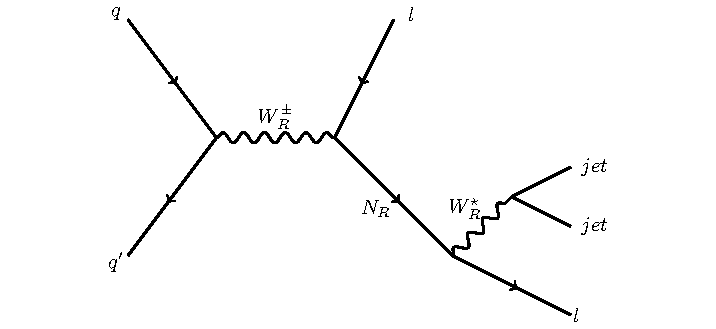
\includegraphics[width=1.0\textwidth]{figures/feynman.pdf}
	\caption{Production of a \WR boson and its decay to two charged leptons and two quarks through 
	a heavy neutrino \nul.}
	\label{fig:wrFeynmanDiagram}
\end{figure}


%%%%%%%%%%%%%%%%%%%%%%%%%%%%%%%%%%%%%%%%%%%%%%%%%%%%%%%%%%%%%%%%%%%%%%%%%%%%%%%%
